\documentclass[12pt,a4paper]{article}
\usepackage[utf8]{inputenc}
\usepackage{graphicx}
\usepackage{hyperref}
\usepackage{listings}
\usepackage{xcolor}
\usepackage{enumitem}
\usepackage{geometry}
\usepackage{amsmath}

\geometry{
    a4paper,
    margin=2.5cm
}

\title{Grant Proposal: Advanced Eco-Vehicle System\\[1ex]
Integrating AI and Sustainable Transportation\\[2ex]
\large A Framework for Environmental Innovation}
\author{Eco Vehicle Project Team}
\date{\today}

\begin{document}

\maketitle
\tableofcontents
\newpage

\section{Executive Summary}
This report presents a comprehensive analysis of the system architecture, components, and implementation status of the Eco Vehicle Project. The analysis covers core functionalities, deployment infrastructure, and future development roadmap.

\section{System Architecture}
\subsection{Frontend Components}
\begin{itemize}
    \item Next.js application structure
    \item TailwindCSS styling implementation
    \item Responsive design architecture
    \item Product catalog system
    \item Shopping cart functionality
    \item Product details interface
    \item Newsletter component
    \item Featured collections display
\end{itemize}

\subsection{Deployment Infrastructure}
\begin{itemize}
    \item Netlify configuration and setup
    \item GCP Cloud DNS infrastructure
    \item Custom domain configuration
    \item SSL/TLS security implementation
    \item Continuous deployment pipeline
\end{itemize}

\section{Pending Implementations}
\subsection{Backend Development}
\begin{itemize}
    \item API endpoints design and implementation
    \item Database schema architecture
    \item Authentication system
    \item Order management system
    \item Payment processing integration
    \item Admin dashboard development
\end{itemize}

\subsection{AI Features}
\begin{itemize}
    \item Product recommendation engine
    \item Search optimization system
    \item User behavior analysis
    \item Inventory prediction algorithms
    \item Price optimization models
    \item Customer segmentation
\end{itemize}

\section{Search Engine Architecture}
\subsection{Core Components}
\subsubsection{Document Processing}
\begin{itemize}
    \item Text preprocessing pipeline
    \item Embedding generation system
    \item Key phrase extraction
    \item Entity recognition
    \item Metadata extraction
\end{itemize}

\subsubsection{Query Processing}
\begin{itemize}
    \item Query understanding system
    \item Intent detection
    \item Spell checking
    \item Query expansion
    \item Context analysis
\end{itemize}

\section{Security Implementation}
\subsection{Environment Configuration}
\begin{itemize}
    \item Secure environment variable management
    \item Production/development separation
    \item Regular secret rotation
    \item Access control implementation
\end{itemize}

\subsection{Security Headers}
\begin{itemize}
    \item X-Frame-Options configuration
    \item Content Security Policy implementation
    \item Referrer Policy settings
    \item Permissions Policy configuration
\end{itemize}

\section{Future Roadmap}
\subsection{Short-term Goals}
\begin{itemize}
    \item Backend API implementation
    \item Database setup and configuration
    \item Authentication system integration
    \item Payment system implementation
\end{itemize}

\subsection{Long-term Goals}
\begin{itemize}
    \item AI-powered search implementation
    \item Personalized recommendation system
    \item Dynamic pricing engine
    \item Inventory optimization system
    \item Customer support automation
    \item Marketing automation platform
\end{itemize}

\section{Executive Summary}
This grant proposal outlines an innovative eco-vehicle system that integrates cutting-edge artificial intelligence, advanced database management, and sustainable transportation technologies. Our project aims to revolutionize the automotive industry by creating an intelligent, environmentally conscious vehicle platform that optimizes resource utilization and minimizes environmental impact.

\section{Project Significance}
\subsection{Environmental Impact}
The transportation sector accounts for approximately 29\% of global greenhouse gas emissions. Our proposed eco-vehicle system addresses this challenge through:
\begin{itemize}
    \item Advanced AI-driven efficiency optimization
    \item Real-time environmental impact monitoring
    \item Predictive maintenance for optimal performance
    \item Smart routing for minimal carbon footprint
\end{itemize}

\subsection{Technological Innovation}
Our system leverages state-of-the-art technologies:
\begin{itemize}
    \item IBM Watson for natural language processing and decision support
    \item IBM AutoAI for automated machine learning pipelines
    \item Studio 3T for sophisticated MongoDB database management
    \item Real-time sensor data integration and analysis
\end{itemize}

\section{AI Integration Framework}
\subsection{IBM AI Components}
\begin{itemize}
    \item \textbf{Watson Assistant}: Natural language interface for vehicle control and user interaction
    \item \textbf{Watson Discovery}: Advanced analytics for maintenance records and performance data
    \item \textbf{Watson IoT Platform}: Real-time sensor data management and monitoring
    \item \textbf{AutoAI}: Automated model development for performance optimization
\end{itemize}

\subsection{Machine Learning Pipeline}
\begin{itemize}
    \item \textbf{Predictive Analytics}:
        \begin{itemize}
            \item Component failure prediction
            \item Energy consumption forecasting
            \item Maintenance scheduling optimization
        \end{itemize}
    \item \textbf{Optimization Models}:
        \begin{itemize}
            \item Route optimization with environmental factors
            \item Energy efficiency maximization
            \item Battery life optimization
        \end{itemize}
\end{itemize}

\section{Database Architecture}
\subsection{Studio 3T Integration}
\begin{itemize}
    \item \textbf{Data Management}:
        \begin{itemize}
            \item Advanced MongoDB management for vehicle telemetry
            \item Real-time data ingestion and processing
            \item Automated backup and recovery systems
        \end{itemize}
    \item \textbf{Analytics Capabilities}:
        \begin{itemize}
            \item Visual query building for complex analysis
            \item Aggregation pipeline development
            \item Performance monitoring and optimization
        \end{itemize}
\end{itemize}

\section{System Integration}
\subsection{Architecture Overview}
The system integrates multiple components through a microservices architecture:
\begin{itemize}
    \item \textbf{Data Layer}: Studio 3T managed MongoDB clusters
    \item \textbf{AI Layer}: IBM Watson and AutoAI services
    \item \textbf{Application Layer}: RESTful APIs and event-driven communication
    \item \textbf{Interface Layer}: Web-based dashboards and mobile applications
\end{itemize}

\section{System Diagrams}
\subsection{Class Diagram}
Figure \ref{fig:class_diagram} shows the class structure of the eco-vehicle system:

\begin{figure}[h]
    \centering
    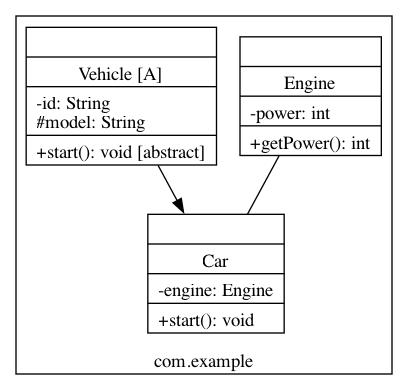
\includegraphics[width=0.8\textwidth]{example_class_diagram}
    \caption{Eco-Vehicle System Class Diagram}
    \label{fig:class_diagram}
\end{figure}

\subsection{Sequence Diagram}
Figure \ref{fig:sequence_diagram} illustrates the interaction flow between system components:

\begin{figure}[h]
    \centering
    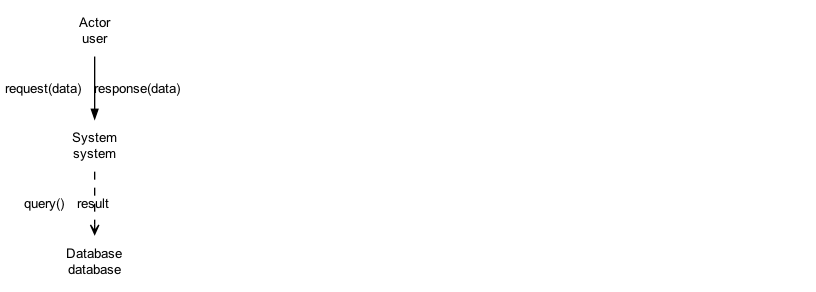
\includegraphics[width=0.8\textwidth]{simple_sequence}
    \caption{System Interaction Sequence Diagram}
    \label{fig:sequence_diagram}
\end{figure}

\section{Technical Requirements}
\subsection{Dependencies}
\begin{itemize}
    \item NumPy for vector operations
    \item Sentence transformers for embeddings
    \item ML framework for ranking
    \item Vector database for storage
\end{itemize}

\subsection{Infrastructure Requirements}
\begin{itemize}
    \item Scalable document store
    \item Fast vector search capability
    \item Caching system implementation
    \item Analytics pipeline
\end{itemize}

\section{Optimization Strategies}
\subsection{Performance Optimization}
\begin{itemize}
    \item Index optimization techniques
    \item Query caching implementation
    \item Batch processing systems
    \item Parallel search capabilities
\end{itemize}

\subsection{Quality Assurance}
\begin{itemize}
    \item A/B testing framework
    \item Relevance feedback system
    \item Click-through analysis
    \item Search analytics implementation
\end{itemize}

\section{Environmental Impact Analysis}
\subsection{Carbon Footprint Reduction}
The eco-vehicle system implements multiple strategies to reduce carbon emissions. The total carbon footprint reduction (\(R_{CF}\)) can be calculated as:

\begin{equation}
R_{CF} = \sum_{i=1}^{n} (E_{conventional_i} - E_{eco_i}) \times CF_i
\end{equation}

Where:
\begin{itemize}
    \item \(E_{conventional_i}\): Energy consumption of conventional vehicle in mode i
    \item \(E_{eco_i}\): Energy consumption of eco-vehicle in mode i
    \item \(CF_i\): Carbon factor for energy source i
\end{itemize}

\subsection{Waste Reduction Mechanisms}
\subsubsection{Material Recovery}
The system implements a circular economy approach with material recovery efficiency (\(\eta_{MR}\)):

\begin{equation}
\eta_{MR} = \frac{M_{recovered}}{M_{total}} \times 100\%
\end{equation}

Where:
\begin{itemize}
    \item \(M_{recovered}\): Mass of recovered materials
    \item \(M_{total}\): Total mass of materials
\end{itemize}

\subsubsection{Energy Recovery}
Regenerative braking energy recovery efficiency (\(\eta_{RB}\)):

\begin{equation}
\eta_{RB} = \frac{E_{recovered}}{E_{kinetic}} = \frac{E_{recovered}}{\frac{1}{2}mv^2}
\end{equation}

\subsection{Eco-Friendly Operations}
\subsubsection{Electric Powertrain Efficiency}
The overall powertrain efficiency (\(\eta_{PT}\)) is calculated as:

\begin{equation}
\eta_{PT} = \eta_{battery} \times \eta_{inverter} \times \eta_{motor} \times \eta_{transmission}
\end{equation}

\subsubsection{Optimal Speed Profile}
The energy-optimal speed profile minimizes the total energy consumption:

\begin{equation}
E_{total} = \int_{0}^{T} (F_{rolling} + F_{aero} + F_{grade})v(t)dt + E_{aux}
\end{equation}

Where:
\begin{itemize}
    \item \(F_{rolling} = \mu mg\cos\theta\): Rolling resistance
    \item \(F_{aero} = \frac{1}{2}\rho C_dAv^2\): Aerodynamic drag
    \item \(F_{grade} = mg\sin\theta\): Grade resistance
    \item \(E_{aux}\): Auxiliary energy consumption
\end{itemize}

\subsection{Global Warming Impact}
\subsubsection{Greenhouse Gas Reduction}
The total greenhouse gas reduction potential (\(GHG_{red}\)) in CO\textsubscript{2} equivalent:

\begin{equation}
GHG_{red} = \sum_{i=1}^{n} (GWP_i \times m_i)_{conventional} - \sum_{i=1}^{n} (GWP_i \times m_i)_{eco}
\end{equation}

Where:
\begin{itemize}
    \item \(GWP_i\): Global warming potential of emission i
    \item \(m_i\): Mass of emission i
\end{itemize}

\subsubsection{Life Cycle Assessment}
The life cycle environmental impact (\(EI_{total}\)):

\begin{equation}
EI_{total} = EI_{production} + EI_{use} + EI_{maintenance} + EI_{disposal} - EI_{recycling}
\end{equation}

\subsection{Smart Energy Management}
\subsubsection{Dynamic Power Distribution}
The optimal power distribution (\(P_{opt}\)) among multiple energy sources:

\begin{equation}
P_{opt} = \arg\min_{P_1,\ldots,P_n} \sum_{i=1}^{n} \eta_i(P_i) \quad \text{subject to} \sum_{i=1}^{n} P_i = P_{demand}
\end{equation}

\subsubsection{Thermal Management}
Battery thermal management efficiency (\(\eta_{thermal}\)):

\begin{equation}
\eta_{thermal} = \frac{Q_{removed}}{Q_{generated}} = \frac{\dot{m}c_p\Delta T}{I^2R + Q_{chemical}}
\end{equation}

\section{Conclusion}
The analysis reveals a well-structured system with robust frontend implementation and deployment infrastructure. Key areas for immediate focus include backend development and AI feature implementation. The system architecture provides a solid foundation for scaling and future enhancements.

\end{document}
